
%(BEGIN_QUESTION)
% Copyright 2011, Tony R. Kuphaldt, released under the Creative Commons Attribution License (v 1.0)
% This means you may do almost anything with this work of mine, so long as you give me proper credit

Les og lag en disposisjon av delkapittelet ``Fresnel Zones'' i delen ``Radio Systems'' i kapittelet ``Wireless Instrumentation'' i læreboken {\it Lessons In Industrial Instrumentation}. Noter sidetall for viktige illustrasjoner, fotografier, ligninger, tabeller og andre relevante detaljer. Forbered deg på å diskutere begreper og eksempler fra lesingen med lærer og medstudenter.

\underbar{file i00549}
%(END_QUESTION)





%(BEGIN_ANSWER)


%(END_ANSWER)





%(BEGIN_NOTES)

RF-energi følger ikke en ren rettlinjet bane fra sendeantenne til mottakerantenne, selv med svært retningsbestemt antenne. I stedet bør vi se det som en serie avlange romvolumer kalt {\it Fresnel-soner}. Radius for Fresnel-sone beregnes slik:

$$r = \sqrt{{n \lambda d_1 d_2} \over D}$$

\noindent
Der,

$r$ = Radius for Fresnel-sonen i punktet av interesse

$n$ = Fresnel-sonenummer (heltall, der 1 er første sone)

$d_1$ = Avstand mellom den ene antennen og punktet av interesse

$d_2$ = Avstand mellom den andre antennen og punktet av interesse

$D$ = Avstand mellom antennene

$$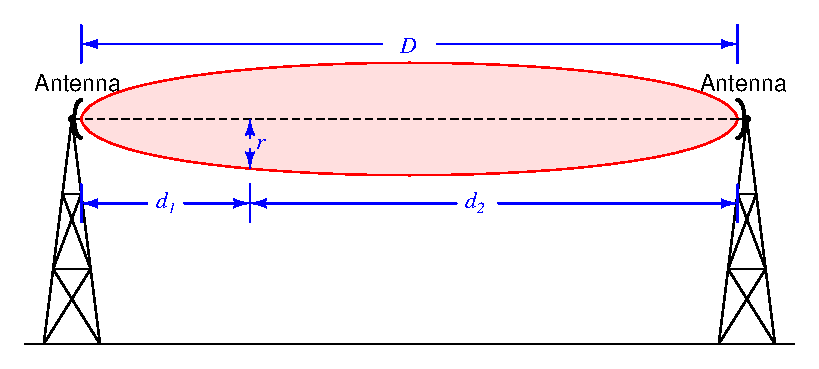
\includegraphics[width=15.5cm]{i00549x01.eps}$$

For mikrobølge-RF er målet at innerste Fresnel-sone ($n=1$) ikke er mer enn 40\% blokkert. Et godt designmål er å unngå all interferens i sone 1. Det er dette fri ``line of sight'' egentlig betyr: at hele den innerste Fresnel-sonen er fri for interferens (inkludert interferens fra bakken).






\vskip 20pt \vbox{\hrule \hbox{\strut \vrule{} {\bf Forslag til sokratisk diskusjon} \vrule} \hrule}

\begin{itemize}
\item{} Forklar hva en {\it Fresnel-sone} er, og hvorfor den er viktig i RF-linkberegninger.
\item{} Øker, minker eller forblir bredden til en Fresnel-sone den samme når signalfrekvensen øker?
\item{} Øker, minker eller forblir bredden til en Fresnel-sone den samme når signalfrekvensen minker?
\item{} Øker, minker eller forblir bredden til en Fresnel-sone den samme når avstanden mellom antennene øker?
\item{} Øker, minker eller forblir bredden til en Fresnel-sone den samme når avstanden mellom antennene minker?
\end{itemize}





\vfil \eject

\noindent
{\bf Prep Quiz:}

As the frequency of a radio signal increases, its Fresnel zone will do what (all other things remaining the same)?

\begin{itemize}
\item{} There will be no effect on the Fresnel zone resulting from a frequency change
\vskip 5pt 
\item{} The maximum width of the Fresnel zone will increase (become fatter)
\vskip 5pt 
\item{} The end-to-end length of the Fresnel zone will increase (become longer)
\vskip 5pt 
\item{} The maximum width of the Fresnel zone will decrease (become skinnier)
\vskip 5pt 
\item{} The end-to-end length of the Fresnel zone will decrease (become shorter)
\vskip 5pt 
\item{} The power density will decrease (the RF energy will ``spread'' more)
\end{itemize}



\vfil \eject

\noindent
{\bf Summary Quiz:}

Calculate the {\it maximum total width} of the first Fresnel zone for two radio antennas operating at 2.4 GHz, separated by a distance of 1400 meters:

\begin{itemize}
\item{} 10.80 meters
\vskip 5pt 
\item{} 43.72 meters
\vskip 5pt 
\item{} 6.612 meters
\vskip 5pt 
\item{} 87.44 meters
\vskip 5pt 
\item{} 21.59 meters
\vskip 5pt 
\item{} 13.22 meters
\end{itemize}


%INDEX% Leseoppgave: Lessons In Industrial Instrumentation, AC-elektrisitet (antenner -- Fresnel-soner)

%(END_NOTES)

